\textbf{Control Water heater using switch and passive controller in IEEE 4 node feeder Jan 06, 2021}
\subsection{objective} 
    \begin{itemize}
        \item Test behavior of water heater when controlled by switch object using NR and FBS solvers.
        \item Test water heater behavior when controlled by passive controller.
        \item Test water heater behavior when shed command is received.
        % \item When switch is open, the water heater SHALL not consume watts, however, water temperature SHALL decrease.
        % \item When switch is closed, water heater SHALL behave normally.
    \end{itemize}
\subsection{outline}
    
    What steps are required?
    \begin{enumerate}
        \item Switch Object
        \begin{itemize}
            \item Set up a switch object in 4 node feeder.
            \item Use player object to control the state of the switch (OPEN OR CLOSED).
            \item Define player object timestamp to be compatible with CLOCK object. 
        \end{itemize}
        \item Passive Controller:\par
        Passive controller utilizes energy market. When prices are high, water heater turns OFF. When prices are low, water heater turns ON.
        \begin{itemize}
            \item Set up auction object.
            \item Set up passive controller.
            \item Set up water heater object as passive controller child.
            \item Set up a .player file so auction object can read from it. (Alternative solution: Prices can be scheduled using schedule object.)
        \end{itemize}
        \item Shed Command:
        \begin{itemize}
            \item Change water heater setpoints during simulation to simulate shed command.
        \end{itemize}
    \end{enumerate}
\subsection{procedures}
    \begin{enumerate}
        \item Switch Object
        \begin{itemize}
            \item switch object is placed in the triplex section of the feeder (between center tapped transformer and triplex node).
            \item Remember, switch object SHALL be placed between link-based nodes. 
            \item Switch object SHALL be used in INDIVIDUAL mode. It won't work with BANKED mode.
            \item Use NR solver. Switch object may behave incorrectly with FBS solver.
        \end{itemize}
        \item Passive Controller:
        \begin{itemize}
            \item Import market module
            \item Set up auction object with prices source file.
            \item Set up a player object that contains prices data. This object is auction object child.
            \item Set up 
        \end{itemize}
        \item Shed command:
        \begin{itemize}
            \item Using schedule object, setpoints are scheduled every 10 minutes.
            \item The water temperature SHALL decrease below the original setpoints. 
        \end{itemize}
    \end{enumerate}
\subsection{parameters}
    \begin{enumerate}
        \item Water Heater parameter (without Shed command):
        \begin{itemize}
        \item Setpoint 120F
        \item Deadband 2F
        \item Volume 50 Gallons
        \item Water demand ELCAP data
        \item heat$\_$mode ELECTRIC
        \end{itemize}
        \item Switch object state:
            \begin{itemize}
                \item At 4:00 pm, switch is CLOSED until 6:00 pm.
                \item Switch state changes to OPEN from 6:05 pm until 8:00 pm.
                \item Switch state changes to CLOSED from 8:05 pm until the end of the simulation.
            \end{itemize}
        \item passive$\_$controller:
            \begin{itemize}
                \item period 600 seconds. (This property SHALL match simulation time)
                \item Control$\_$mode PROBABILITY$\_$OFF. (SHALL be used when der is aggregated.)
                \item comfort$\_$level SHALL be set to a high number to force water heater to turn OFF at specified times.
                \item state$\_$ property SHALL be override. This is important to force water heater object to stick to parent object parameter.
            \end{itemize}
    \end{enumerate}
\subsection{observations}
    \begin{enumerate}
        \item Switch object:
        \begin{itemize}
            \item Water heater did not respond to switch changes with NR solver.
            \item When switch is open, water heater still turns ON and consume power (kW).
    \end{itemize}
        \item passive$\_$controller:
        \begin{itemize}
            \item water heater behaves as expected.
        \end{itemize}
        \item shed$\_$command
        \begin{itemize}
            \item Setpoints changed as expected.
        \end{itemize}
    \end{enumerate}
\newpage
    
\subsection{data}
    \begin{enumerate}
        \item Switch$\_$object:
        
    
\begin{table}[h]
\begin{tabular}{|l|l|l|l|l}

\cline{1-4}
Timestamp & power (kW) & water$\_$demand (gpm) & is$\_$waterheater$\_$on & \\ \cline{1-4}
2020-01-01 18:00:00 PST & +0 & +0 & 0 & \\ \cline{1-4}
2020-01-01 18:10:00 PST & 0 & 0.16 & 0 &  \\ \cline{1-4}
2020-01-01 18:20:00 PST & 4.5 & 0 & 1 &  \\ \cline{1-4}
\end{tabular}
\caption{Water heater controlled by a switch}
\label{table:1}
\end{table}
        \item passive$\_$controller \newline
        glm file can be found here: \url{https://github.com/psu-powerlab/GridLab-D/blob/master/NeoChargeProject/WH_4_Node_Feeder/Controlled_WH/Controlled_WH_4.glm} \newline \par
        
        Full output file is uploaded to power lab github account: \url{https://github.com/psu-powerlab/GridLab-D/blob/master/NeoChargeProject/WH_4_Node_Feeder/Controlled_WH/wh_1.csv}
        
        \begin{table}[h]
        \begin{tabular}{|l|l|l|l|l}
        \cline{1-4}
        Timestamp & power (kW) & water$\_$demand (gpm) & is$\_$waterheater$\_$on & \\ \cline{1-4}
        2020-01-01 16:00:00 PST & +0 & +0 & 0 & \\ \cline{1-4}
        2020-01-01 16:10:00 PST & +0 & +0 & 0 &  \\ \cline{1-4}
        2020-01-01 16:20:00 PST & +0 & +0 & 0 &  \\ \cline{1-4}
        2020-01-01 16:30:00 PST & +0 & +0 & 0 &  \\ \cline{1-4}
        2020-01-01 16:40:00 PST & +0 & +0 & 0 &  \\ \cline{1-4}
        2020-01-01 16:50:00 PST & +0 & +0.25 & 0 &  \\ \cline{1-4}
        \end{tabular}
        \caption{Water heater controlled by passive controller}
        \label{table:2}
        \end{table}
        
        \item shed$\_$command \newline
        glm file can be found here \url{https://github.com/psu-powerlab/GridLab-D/blob/master/NeoChargeProject/WH_4_Node_Feeder/Controlled_WH/WH_Shed_command.glm} \newline \par
         Full data is uploaded to PSU power lab GitHub account \url{https://github.com/psu-powerlab/GridLab-D/blob/master/NeoChargeProject/WH_4_Node_Feeder/Controlled_WH/wh_shed.csv}\newline \par Does the shed command contain starting and ending time? 
        
        \begin{table}[h]
        \begin{tabular}{|l|l|l|l|l|l}
        \cline{1-5}
        Timestamp & power (kW) & water$\_$demand (gpm) & water$\_$temperature (F) & is$\_$waterheater$\_$on & \\ \cline{1-5}
        2020-01-01 18:00:00 PST & 0 & 0 & 119.008 & 0 & \\ \cline{1-5}
        2020-01-01 18:10:00 PST & 0 & 0.16 & 118.944 & 0 &  \\ \cline{1-5}
        2020-01-01 18:20:00 PST & 0 & 0 & 117.026 & 0 &  \\ \cline{1-5}
        2020-01-01 18:30:00 PST & 0 & 0 & 116.965 & 0 &  \\ \cline{1-5}
        2020-01-01 18:40:00 PST & 0 & 0 & 116.904 & 0 &  \\ \cline{1-5}
        2020-01-01 18:50:00 PST & 0 & 0 & 116.843 & 0 &  \\
        \cline{1-5}
        \end{tabular}
        \caption{Water heater controlled with shed command}
        \label{table:3}
        \end{table}
    \end{enumerate}
\subsection{results}
    \begin{enumerate}
        \item switch$\_$object

        The above table \ref{table:1} is a portion of the water heater output file. At the specified timestamps, the switch is open. It can be seen from the last row that the water heater was turned ON and consumed 4.5 kW even though switch was open. I sent a request to GridLAB-D folks regarding this issue. I will resume this work on switch object once I receive a response. Alternatively, a passive controller object was used. The results are shown in table \ref{table:2}.
    
        \item passive$\_$controller
        
        A shed command is received at 17:00. The water heater is supposed to turn ON at 18:20 as the water temperature drops below the range (118F). Due to shed command, the water temperature continues to drop as shown in table \ref{table:3}.
        \begin{figure}[hbt!]
            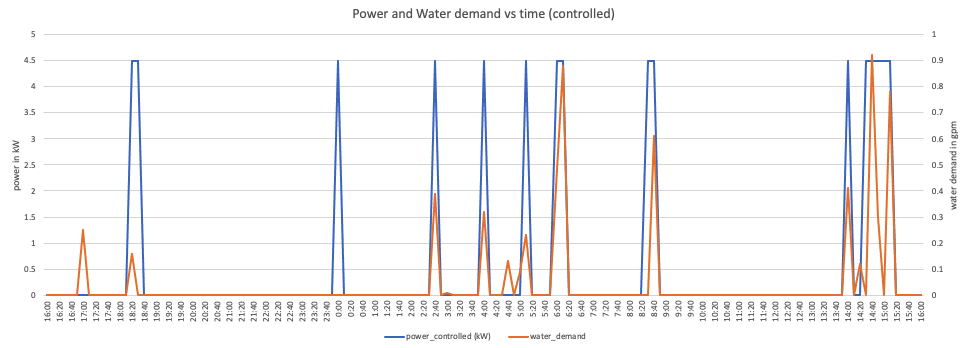
\includegraphics[scale=0.5]{controlled_WH.png}
            \caption{Power and Water Demand vs Time (controlled)}
            \label{fig:controlled_wh}
        \end{figure}
        \newpage
        \item shed$\_$command
        Refer to powerLab github account for glm file and procedure in this link \href{https://github.com/MidrarAdham/GridLab-D/tree/master/NeoChargeProject/WH_4_Node_feeder/WH_shed_command}{Shed Command in EWH}.
        
    \end{enumerate}
    \newpage
